Data from the four experiments were recorded and plotted in figures. The results were analyzed to propose mixing settings.

\begin{figure}[h] %Comparison between all
	\centering
	\begin{tikzpicture}[scale=0.8]
	\begin{axis}[axis x line = bottom, axis y line=left,
	title={Rotational Speed vs. Mixing time}, xlabel=Rotational Speed (RPM), ylabel=Mixing time (S), domain=0:500, ymin=0, ymax=14
	]
	\addplot[red] table[x={Rotational-Speed}, y={Paddle-Mixing-time}]{Mixing-data-1.dat};
	\addplot[blue] table[x={Rotational-Speed}, y={Pitched-blade-Mixing-time}]{Mixing-data-1.dat};
	\addplot[green] table[x={Rotational-Speed}, y={Rushton-mixing-time}]{Mixing-data-1.dat};
	\legend{Paddle, Pitched-blade, Rushton}
	\end{axis}
	\end{tikzpicture}	
	\caption{Rotational speed against liquid mixing time for paddle, pitched-blade, and Rushton turbine.}
	\label{fig:RotationalSpeed-MixingTime}
\end{figure}

According to Figure \ref{fig:RotationalSpeed-MixingTime}, the minimum of each curve indicates the least mixing time for each impeller. Overall, Paddle’s mixing time is longer than that of Pitched-blade or Rushton for the various rotational speed tested. Thus, paddle has been eliminated from our choices of impellers. Comparing the curves of Pitched-blade to Rushton turbine, Pitch-blade achieves mixing under less time for all rotational speeds. This observation is consistent with our hypothesis that Pitched-blade would give the smallest mixing time due to its large impeller diameter. Both Pitched-blade and Rushton reach minimum mixing time at 280rpm, indicating that 280 is the optimal rotational speed that will be used in the final set up.

\begin{figure}[h] %Combinatination of Rushton
	\centering
	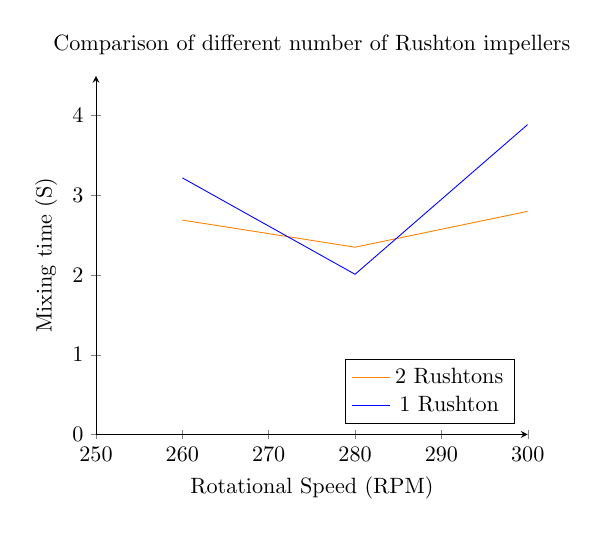
\begin{tikzpicture}[scale=0.8]
	\begin{axis}[axis x line = bottom, axis y line=left,
	title={Comparison of different number of Rushton impellers}, xlabel=Rotational Speed (RPM), ylabel=Mixing time (S), xmin=250,
	ymin=0, ymax=4.5, legend pos = south east
	]
	\addplot[orange] table[]{
		260	2.69
		280	2.35
		300	2.80
	};
	\addplot[blue] table[]{
		260	3.22
		280 2.01
		300 3.89
	};
	\legend{2 Rushtons, 1 Rushton}
	\end{axis}
	\end{tikzpicture}	
	\caption{Rotational speed against liquid mixing time for paddle, pitched-blade, and Rushton turbine.}
	\label{fig:Rushton-comparison}
\end{figure}
\begin{figure}[h] %Different combinations
	\centering
	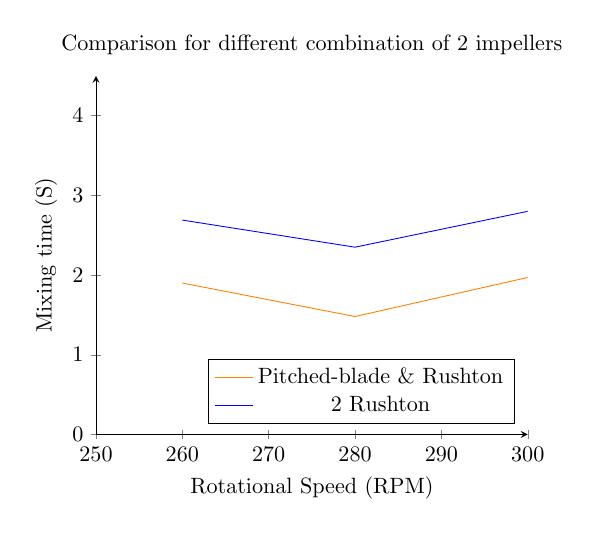
\begin{tikzpicture}[scale=0.8]
	\begin{axis}[axis x line = bottom, axis y line=left,
	title={Comparison for different combination of 2 impellers}, xlabel=Rotational Speed (RPM), ylabel=Mixing time (S), xmin=250,
	ymin=0, ymax=4.5, legend pos = south east
	]
	\addplot[orange] table[]{
		260	1.90
		280	1.48
		300	1.97
	};
	\addplot[blue] table[]{
		260	2.69
		280	2.35
		300	2.80
	};
	\legend{Pitched-blade \& Rushton, 2 Rushton}
	\end{axis}
	\end{tikzpicture}	
	\caption{Comparison of 1 Rushton \& 1 Pitched-blade and 2 Rushtons under unbaffled conditions}
	\label{fig:PitchedAndRushton_2Rushton}
\end{figure}
According to Figure \ref{fig:Rushton-comparison}, 2 Rushton turbines take longer time to achieve homogeneity than 1 Rushton turbine. This result differs from our expectation that 2 impellers would be more effective. One explanation could be that when more impellers are used, larger vortex is generated, and since this experiment is conducted under unbaffled condition, vortex would hinder the mixing, hence slow down mixing time.

Figure \ref{fig:PitchedAndRushton_2Rushton} shows that when 2 impellers are used, the combination of 1 Rushton and 1 Pitched-blade is the most ideal since is achieves a homogeneous solution in the shortest amount of time. It is distinctive that the liquid mixing time of this combination is less than that of any other settings in the previous experiments. This figure also reassures that 280rpm is the optimal rotational speed because both curves reach minimum mixing time at 280rpm.

\begin{figure}[h] %Different combinations
	\centering
	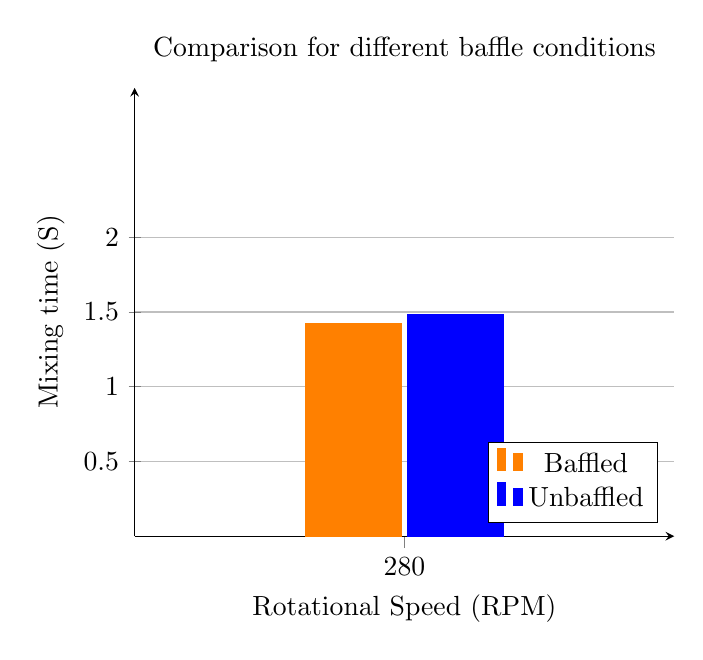
\begin{tikzpicture}
	\begin{axis}[axis x line = bottom, axis y line=left,
	title={Comparison for different baffle conditions}, xlabel=Rotational Speed (RPM), ylabel=Mixing time (S), xtick=data,
	ymin=0, ymax=3, ybar, bar width=20, legend pos = south east, ymajorgrids,
	ytick={0.50, 1.00, 1.50, 2.0}
	]
	\addplot[color=orange, fill=orange] table[]{
		280 1.42
	};
	\addplot[color=blue, fill=blue] table[]{
		280 1.48
	};
	\legend{Baffled, Unbaffled}
	\end{axis}
	\end{tikzpicture}	
	\caption{Liquid mixing time of Rushton turbine under baffled and unbaffled conditions at 280rpm. }
	\label{fig:BaffledVsUnbaffled}
\end{figure}

Figure \ref{fig:BaffledVsUnbaffled} demonstrates that baffles help reducing mixing time as the baffled setting achieves homogeneity in 1.42 seconds whereas it is 1.48 for the unbaffled.  

The design and dimensions of our bioreactor prototype as well as impeller layout are discussed below. 
\begin{enumerate}
	\item Mixing vessel (bench-scale reactor)
	\begin{itemize}
		\item Upper diameter = 10cm
		\item Bottom diameter = 6cm
		\item Height = 12cm; however, we used a maximum \textbf{filling height} of 10cm to allow for the increased volume during stirring.
	\end{itemize}
	\item Baffle dimensions:
	Optimal ratio of baffle width to cup diameter is 1/10 - 1/12 \cite[p.258]{Doran2012}, therefore, the width of baffle is $\frac{1}{10} \cdot \SI{10}{\centi\meter}$. We chose to account for the diameter at the top as the vortex is the greatest there. Based on real life examples, the thickness of a baffle is typically 1/100 the length of the baffle, which is $ \frac{1}{100} \cdot \SI{10}{\centi\meter} = \SI{1}{\milli\meter} (\SI{0.1}{cm})$. This is unrealistically thin for a scale-down of this magnitude hence a thickness of 0.3cm was used.
	\item Impeller layout:
	Two impellers were used. The first, Rushton, is 2.5cm from the top of the stirrer in the cup because to achieve optimal mixing, the distance between the bottom of the tank and the impeller should equal to the diameter of the impeller which in this case is 2.5cm \cite[p.286]{Doran2012} The second impeller, Pitched-blade was placed 4.0cm away from the center of the Rushton since the distance between the two impellers should equal to the diameter of the pitched-blade, 4.0cm \cite[p.286]{Doran2012}.
	\item Volume of water used:
	The maximum height of liquid should be 1.25 times the bottom diameter of vessel which is $1.25\cdot6 = 7.5\si{\centi\meter}$ \cite[p.257]{Doran2012}. Since the height of the magnetic stirrer is 1cm, the maximum height is 7.5 + 1 = 8.5cm from the bottom of the vessel. This is equivalent to a liquid volume of 312mL. A liquid volume of 300ml was used because this value was a good compromise between the maximum solution volume of 315ml and the requirement of a value to easily work with calibration curves. 
\end{enumerate}